\section{Glavne funkcije}
Razvojna plošča vključuje RGB LED, gumb, senzor osvetlitve z možnostjo zamenjave pull-down uporov za zmanjšanje tolerance senzorja, UART, I2C, WiFi, BLE in serijsko komunikacijo. Primerna je za IoT projekte in projekte, ki temeljijo na merjenju in upravljanju glede na ambientalno svetlobo.

\section{Programiranje in okolje}
Programiranje te razvojne plošče poteka preko Arduino IDE, ki je dostopen na \url{https://www.arduino.cc/en/software/}. Poleg tega je treba namestiti še paket plošč esp32.

\subsection{Namestitev paketa esp32}
Za namestitev paketa esp32 pojdite na Tools→Board→Board Manager ali kliknite ikono na levi strani. Poiščite "esp32 by Espressif Systems" in kliknite Install. Če je bilo uspešno nameščeno, se bo pod Tools→Board pojavila možnost esp32, znotraj katere so vse esp32 plošče, vključno z ESP32C3 Dev Module, ki je naša plošča.

\begin{figure}[H]
    \centering
    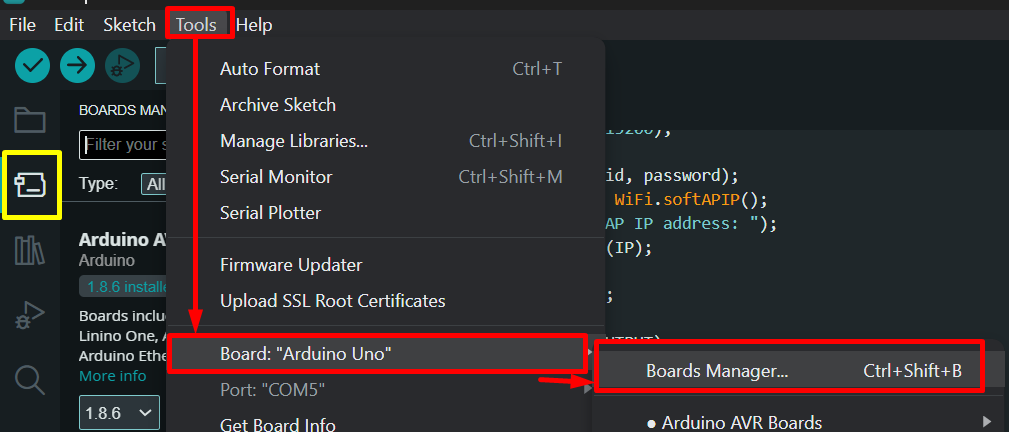
\includegraphics[width=0.9\linewidth]{Imgs/boardsetup1.png}
    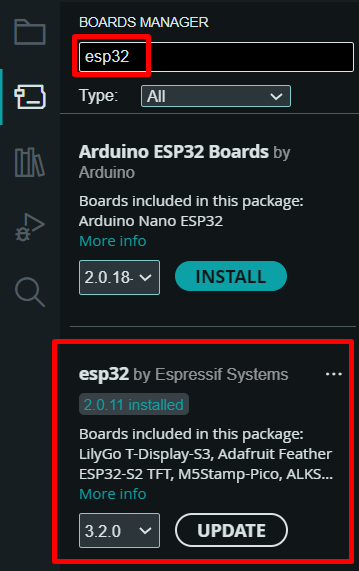
\includegraphics[width=0.5\linewidth]{Imgs/boardsetup2.png}
    \caption{Namestitev paketa esp32}
    \label{fig:enter-label}
\end{figure}

\subsection{Postopek nalaganja programa}
Za nalaganje programa na ploščo jo priključite preko USB-ja, preverite da so nastavitve plošče ustrezne (spodaj navedene), in kliknite Upload. Ko piše "done uploading", lahko ploščo odklopite.
Board settings: 
\begin{enumerate}
    \item Board: ESP32C3 Dev Module
    \item Port: ustrezen COM port
    \item USB CDC On Boot: Enabled 
    \item CPU Frequency: 80MHz
\end{enumerate}

\section{Pomembni pini}
\begin{enumerate}
    \item Gumb: 9
    \item Rdeča LED: 7
    \item Zelena LED: 10
    \item Modra LED: 4
    \item LX\_A: 1
    \item LX\_B: 3
    \item LX\_OUT: 0
    \item SDA: 5
    \item SCL: 6
    \item RX: 20
    \item TX: 21
\end{enumerate}

\section{Uporaba light sensorja}
Z zamenjavo stanj pinov LX\_A in LX\_B na HIGH ali LOW(to lahko naredite tudi ročno s spreminjanjem uporov prek jumperjev) lahko spreminjate občutljivost svetlobnega senzorja. Spodaj je primer kode, kjer lahko z izbiro mode 1, 2 ali 3 spreminjate območje izmerjene izhodne napetosti.

\begin{lstlisting}[language=Arduino]
#define LX_A 1
#define LX_B 3
#define LX_OUT 0

void setup() {
  Serial.begin(115200);

  pinMode(LX_A, OUTPUT);
  pinMode(LX_B, OUTPUT);
  pinMode(LX_OUT, INPUT);

  Serial.println("Select mode:");
  Serial.println("Mode 1");
  Serial.println("Mode 2");
  Serial.println("Mode 3");
}

void loop() {
  if (Serial.available() > 0) {
    char c = Serial.read();

    switch (c) {
      case '1':  // Mode 1
        digitalWrite(LX_A, LOW);  
        digitalWrite(LX_B, LOW);  
        Serial.println("Mode set to 1");
        break;
      case '2':  // Mode 2
        digitalWrite(LX_A, LOW); 
        digitalWrite(LX_B, HIGH);
        Serial.println("Mode set to 2");
        break;
      case '3':  // Mode 3
        digitalWrite(LX_A, HIGH);  
        digitalWrite(LX_B, LOW); 
        Serial.println("Mode set to 3");
        break;
    }
  }

  int output = analogRead(LX_OUT);

  Serial.println(output);

  delay(100);
}
\end{lstlisting}

\section{Primeri funkcije}
\subsection{RGB LED}
Povezava do knjižnice: \url{https://docs.arduino.cc/language-reference/en/functions/digital-io/digitalwrite/}
\begin{lstlisting}[language=Arduino]  
#define LED_R 7
#define LED_G 10
#define LED_B 4

void setup() {
  pinMode(LED_R, OUTPUT);
  pinMode(LED_G, OUTPUT);
  pinMode(LED_B, OUTPUT);
}

void loop() {
  analogWrite(LED_R, 255); // red
  analogWrite(LED_G, 0);
  analogWrite(LED_B, 0);
  delay(1000);

  analogWrite(LED_R, 0);
  analogWrite(LED_G, 255); // green
  analogWrite(LED_B, 0);
  delay(1000);

  analogWrite(LED_R, 0);
  analogWrite(LED_G, 0);
  analogWrite(LED_B, 255); // blue
  delay(1000);
}
\end{lstlisting}

\subsection{Gumb}
Povezava do knjižnice: \url{https://docs.arduino.cc/language-reference/en/functions/digital-io/digitalread/}
\begin{lstlisting}[language=Arduino]  
#define BTN 9
#define LED_R 7

void setup() {
  pinMode(BTN, INPUT_PULLUP);
  pinMode(LED_R, OUTPUT);
}

void loop() {
  if (digitalRead(BTN) == LOW) {
    digitalWrite(LED_R, HIGH); // button pressed
  } else {
    digitalWrite(LED_R, LOW);
  }
}    
\end{lstlisting}

\subsection{Light sensor}
Povezava do knjižnice: \url{https://docs.arduino.cc/language-reference/en/functions/analog-io/analogRead/}
\begin{lstlisting}[language=Arduino]  
#define LX_A 1
#define LX_B 3
#define LX_OUT 0

void setup() {
  Serial.begin(115200);
  delay(300);
}

void loop() {
  int lightLevel = lx(1);
  Serial.print("Light Level: ");
  Serial.println(lightLevel);
  delay(500);
}

int lx(int mode) {
  switch (mode) {
    case 0:
      pinMode(LX_A, INPUT);
      pinMode(LX_B, INPUT);
      break;
    case 1:
      pinMode(LX_A, INPUT);
      pinMode(LX_B, OUTPUT);
      digitalWrite(LX_B, LOW);
      break;
    case 2:
      pinMode(LX_A, OUTPUT);
      digitalWrite(LX_A, LOW);
      pinMode(LX_B, INPUT);
      break;
    default:
      pinMode(LX_A, INPUT);
      pinMode(LX_B, INPUT);
  }

  return analogRead(LX_OUT);
}
\end{lstlisting}

\subsection{Serial komunikacija}
Povezava do knjižnice: \url{https://www.arduino.cc/reference/en/language/functions/communication/serial/}
\begin{lstlisting}[language=Arduino]  
void setup() {
  Serial.begin(115200);
  delay(1000);
  Serial.println("Serial is working!");
}

void loop() {
  if (Serial.available()) {
    String input = Serial.readStringUntil('\n');
    Serial.print("You said: ");
    Serial.println(input);
  }
}
\end{lstlisting}

\subsection{Wi-fi}
Povezava do knjižnice: \url{https://docs.arduino.cc/libraries/wifi/}
\begin{lstlisting}[language=Arduino]  
#include <WiFi.h>

const char* ssid = "SSID";
const char* password = "PASSWD";
WiFiServer server(80);

void setup() {
  Serial.begin(115200);
  delay(1000);

  Serial.print("Connecting to ");
  Serial.println(ssid);
  WiFi.begin(ssid, password);

  while (WiFi.status() != WL_CONNECTED) {
    delay(500);
    Serial.print(".");
  }

  Serial.println("");
  Serial.println("WiFi connected.");
  Serial.print("IP address: ");
  Serial.println(WiFi.localIP());

  server.begin();
}

void loop() {
  WiFiClient client = server.available(); 

  if (client) {
    Serial.println("New Client.");
    String request = client.readStringUntil('\r');
    Serial.println(request);
    client.flush();

    client.println("HTTP/1.1 200 OK");
    client.println("Content-type:text/html");
    client.println();
    client.println("<!DOCTYPE html><html><body><h1>Mehatronika</h1></body></html>");
    client.println();
    client.stop();
    Serial.println("Client disconnected.");
  }
}
\end{lstlisting}

\subsection{Bluetooth}
Povezava do knjižnice: \url{https://github.com/nkolban/ESP32_BLE_Arduino}
\begin{lstlisting}[language=Arduino]  
#include <BLEDevice.h>
#include <BLEUtils.h>
#include <BLEServer.h>

#define SERVICE_UUID        "4fafc201-1fb5-459e-8fcc-c5c9c331914b"
#define CHARACTERISTIC_UUID "beb5483e-36e1-4688-b7f5-ea07361b26a8"

void setup() {
  Serial.begin(115200);
  Serial.println("Starting BLE work!");

  BLEDevice::init("Long name works now");
  BLEServer *pServer = BLEDevice::createServer();
  BLEService *pService = pServer->createService(SERVICE_UUID);
  BLECharacteristic *pCharacteristic = pService->createCharacteristic(
                                         CHARACTERISTIC_UUID,
                                         BLECharacteristic::PROPERTY_READ |
                                         BLECharacteristic::PROPERTY_WRITE
                                       );

  pCharacteristic->setValue("Hello World says Neil");
  pService->start();
  BLEAdvertising *pAdvertising = BLEDevice::getAdvertising();
  pAdvertising->addServiceUUID(SERVICE_UUID);
  pAdvertising->setScanResponse(true);
  pAdvertising->setMinPreferred(0x06);
  pAdvertising->setMinPreferred(0x12);
  BLEDevice::startAdvertising();
  Serial.println("Characteristic defined! Now you can read it in your phone!");
}
\end{lstlisting}

\subsection{I2C}
Povezava do knjižnice: \url{https://www.arduino.cc/en/Reference/Wire}
\begin{lstlisting}[language=Arduino]  
#include <Wire.h>
#define SDA 5
#define SCL 6

void setup() {
  Wire.begin(SDA, SCL);
  Serial.begin(115200);
  delay(1000);
  Serial.println("I2C Scanner starting...");

  for (uint8_t address = 1; address < 127; ++address) {
    Wire.beginTransmission(address);
    if (Wire.endTransmission() == 0) {
      Serial.print("I2C device found at address 0x");
      Serial.println(address, HEX);
    }
    delay(5);
  }

  Serial.println("Scan complete.");
}
\end{lstlisting}

\subsection{UART}
Povezava do knjižnice: \url{https://docs.arduino.cc/learn/communication/uart/}
\begin{lstlisting}[language=Arduino]
#define RX 20
#define TX 21

void setup() {
  Serial.begin(115200);               // USB Serial Monitor
  Serial1.begin(9600, SERIAL_8N1, RX, TX); // UART Serial
  Serial.println("UART echo demo started...");
}

void loop() {
  if (Serial1.available()) {
    char c = Serial1.read();     // Read from UART
    Serial1.write(c);            // Echo back to UART
    Serial.print("Received: ");
    Serial.println(c);           // Also print to USB serial for debugging
  }
}

\end{lstlisting}



